\documentclass[a4paper,12pt]{article}
\usepackage[MeX]{polski}
\usepackage[utf8]{inputenc}
\usepackage{graphicx}

%opening
\title{Treffort-Cuisiat}
\author{Michał Kozłowski}

\begin{document}

\maketitle

%\begin{abstract}

%\end{abstract}


\section{,,Opis''}

\begin{figure}
\centering
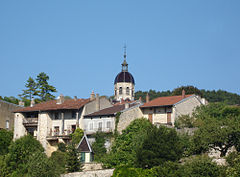
\includegraphics[width=0.5\textwidth]{grafika/obrazek.jpg}
\caption{Treffort-Cuisiat (2009)}
\label{fig:fotografia}
\end{figure}

Treffort-Cuisiat (zob. zdjęcie (\ref{fig:fotografia})) --- miejscowość i~dawna gmina we~Francji, w~regionie Owernia-Rodan-Alpy, w~departamencie Ain. W~dniu 1~stycznia~2016~roku z~połączenia dwóch ówczesnych gmin – Pressiat oraz~Treffort-Cuisiat – powstała nowa gmina Val-Revermont. Siedzibą gminy została miejscowość Treffort-Cuisiat. W 2013 roku populacja Treffort-Cuisiat wynosiła 2334 mieszkańców. 



\begin{table}
\centering
\begin{tabular}{lc}
\textbf{Dane}&\textbf{Informacje}\\
\hline
Państwo&Francja\\
Region&Owernia-Rodan-Alpy\\
Departament&Ain\\
Okręg&Bourg-en-Bresse\\
Kanton&Saint-Étienne-du-Bois\\
Kod&INSEE	01426\\
Mer&Monique Wiel (2014-2020)\\
Powierzchnia&39,41 km$^2$\\
Wysokość&221-681 m n.p.m.\\
Populacja (2013)&2334\\
Kod pocztowy&01370\\
\hline
\end{tabular}
\caption{Ogólne informacje}
\end{table}



\begin{table}
\centering
\begin{tabular}{lc}
\textbf{rok} & \textbf{zaludnienie}\\
\hline
1962 & 1233\\
1968 & 1167\\
1975 & 1101\\
1982 & 1556\\
1990 & 1779\\
1999 & 1910\\
2008 & 2070\\
\hline
\end{tabular}

\caption{Populacja Treffort-Cuisiat w latach 1962–2008}
\end{table}


\end{document}